\documentclass{article}
\usepackage{amssymb} % checkmark
\usepackage{graphicx}
\graphicspath{ {./resources/} }
\usepackage[justification=justified,singlelinecheck=false]{caption}
\usepackage[dvipsnames]{xcolor} % color and naming extension
% \definecolor{lgcustom}{rgb}{83, 83, 83} % don't work
\newcommand{\ccheck}[1]{\textcolor{ForestGreen}{\emph{(\checkmark #1)}}} % marking completed task
\usepackage{typed-checklist} % todo list
\usepackage{float} % improves image positioning
\usepackage{multirow}
\usepackage{minted} % code syntax highlighting
\usepackage{url} %bibtex
\usepackage{hyperref} %bibtex

\title{Assignment 2 UFO \\ \LaTeX\ \\ Task 2 - Bachelor Template}
\date{07-03-2021}
\author{Rúni Vedel Niclasen}

\begin{document}

\maketitle
\thispagestyle{empty} % no numbering [first page] (better than gobble)
\ccheck{Title page without page number}

\newpage
\thispagestyle{empty} % no numbering [third page] (better than gobble)
\tableofcontents
\ccheck{Table of contents}

\newpage
\pagenumbering{arabic}

\section{Danish characters: æ, ø, å}
Test case: Rød grød med fløde\\
Test case 2: RØD GRØD MED FLØDE

\ccheck{Danish characters}

\section{Graphics}

\subsection{Caption over image}
\begin{figure}[H]
    \caption{\ccheck{Caption above}} % left-align done by caption package at top
    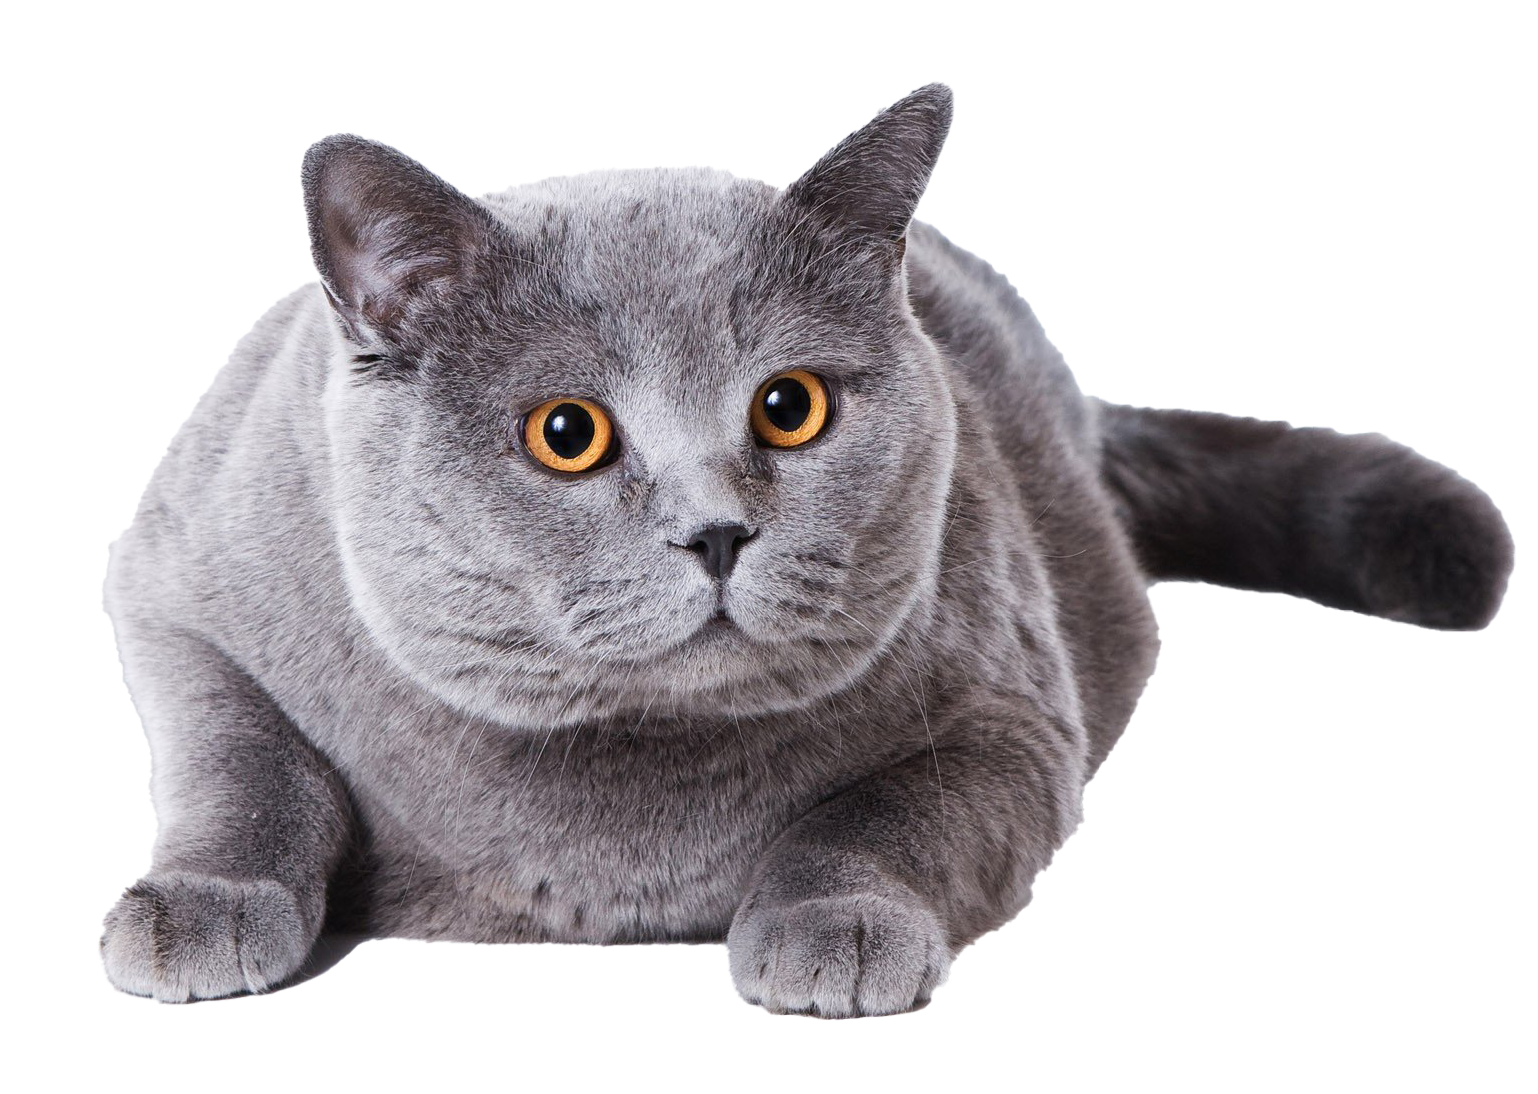
\includegraphics[scale=0.3]{catpng}
\end{figure}

\subsection{Caption under image}
\begin{figure}[H]
    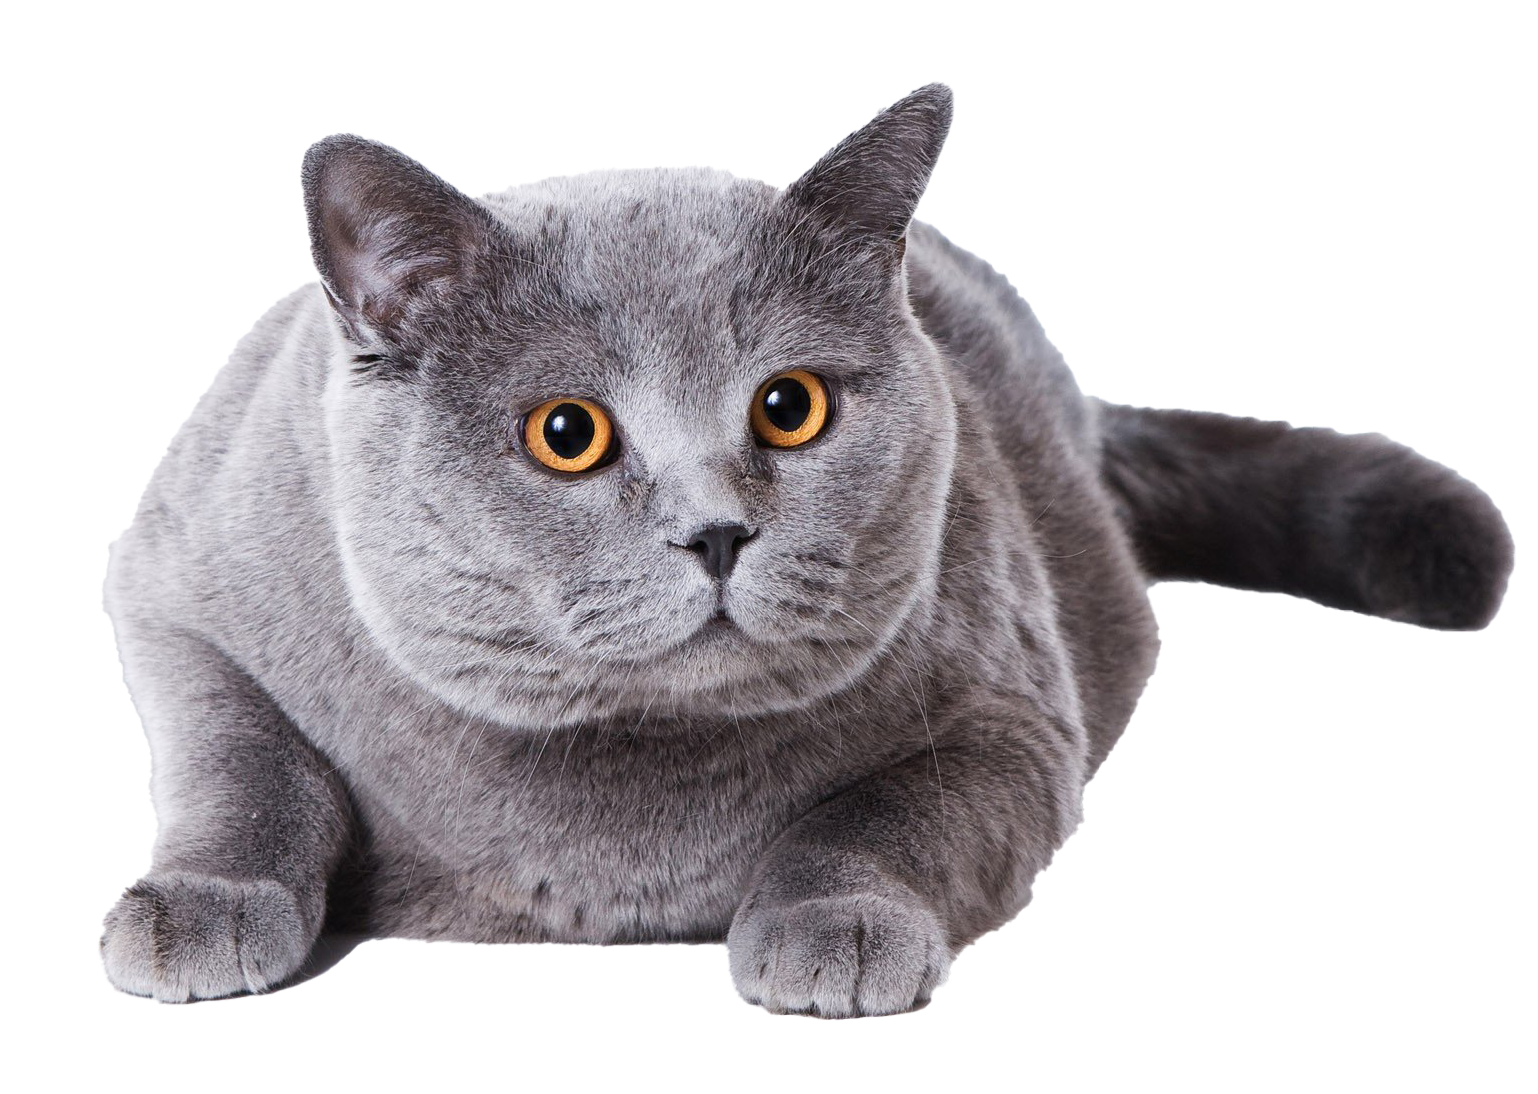
\includegraphics[scale=0.3, angle=180]{catpng}
    \caption{\ccheck{Caption under}} % left-align done by caption package at top
\end{figure}

\subsection{With label}
\begin{figure}[H]
    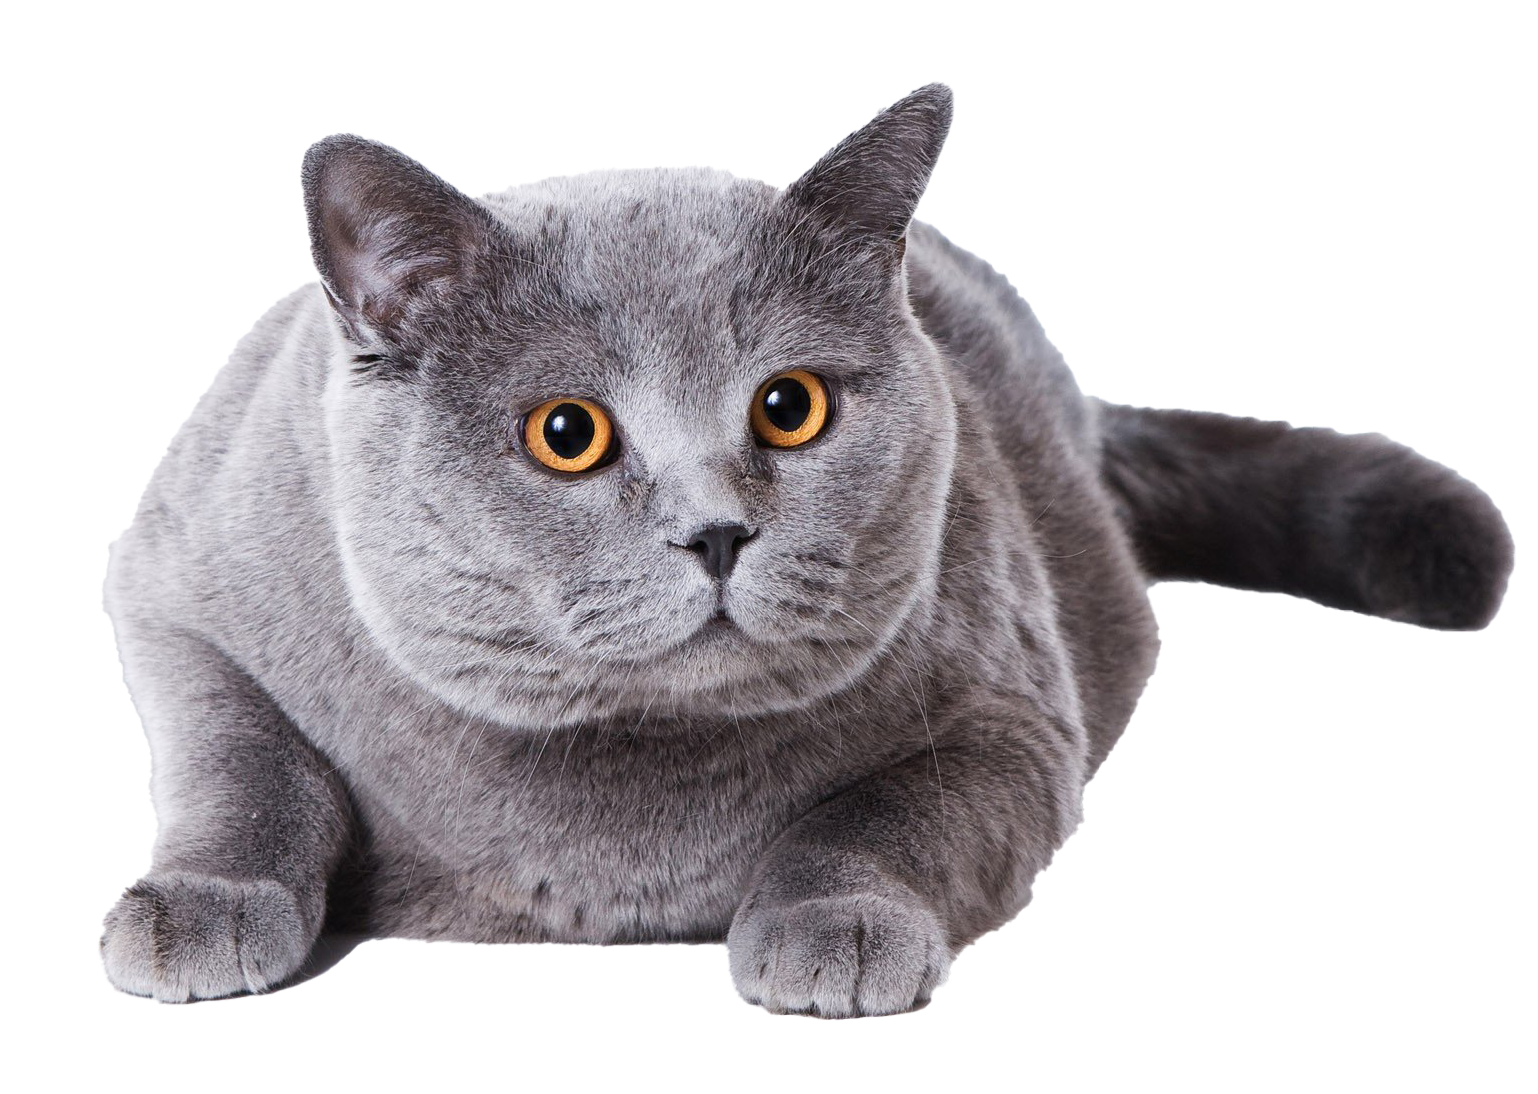
\includegraphics[scale=0.3, angle=45]{catpng}
    \caption{\ccheck{With label} (labelcat)}
    \label{fig: labelcat}
Here [\ref{fig: labelcat}] is a direct reference to the above cat, aptly named \emph{labelcat}.
\end{figure}

\subsection{Centered}
\begin{figure}[h]
    \centering
    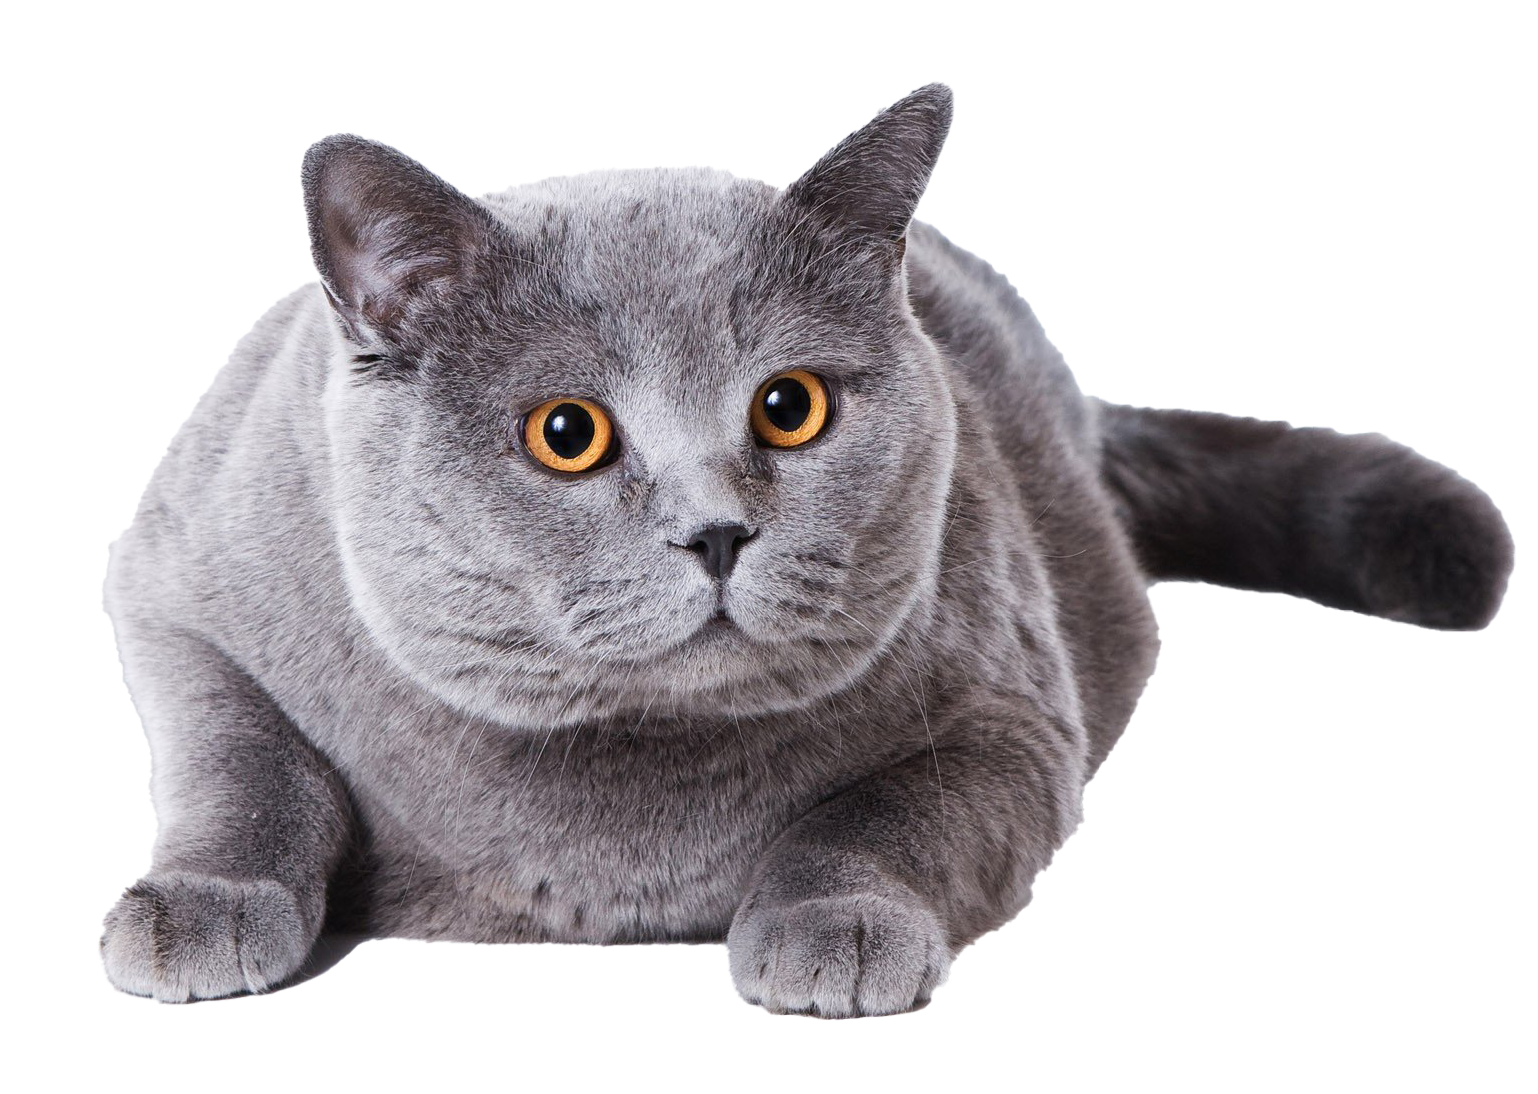
\includegraphics[width=12cm, height=3cm]{catpng}
    \captionsetup{justification=centering}
    \caption{\ccheck{Centered image} (wide cat)} % left-align done by caption package at top
    \label{fig: centercat}
\end{figure}


\subsection{Two images next to each other}
\begin{figure}[H]
    \centering
    \begin{minipage}[b]{0.4\textwidth}
      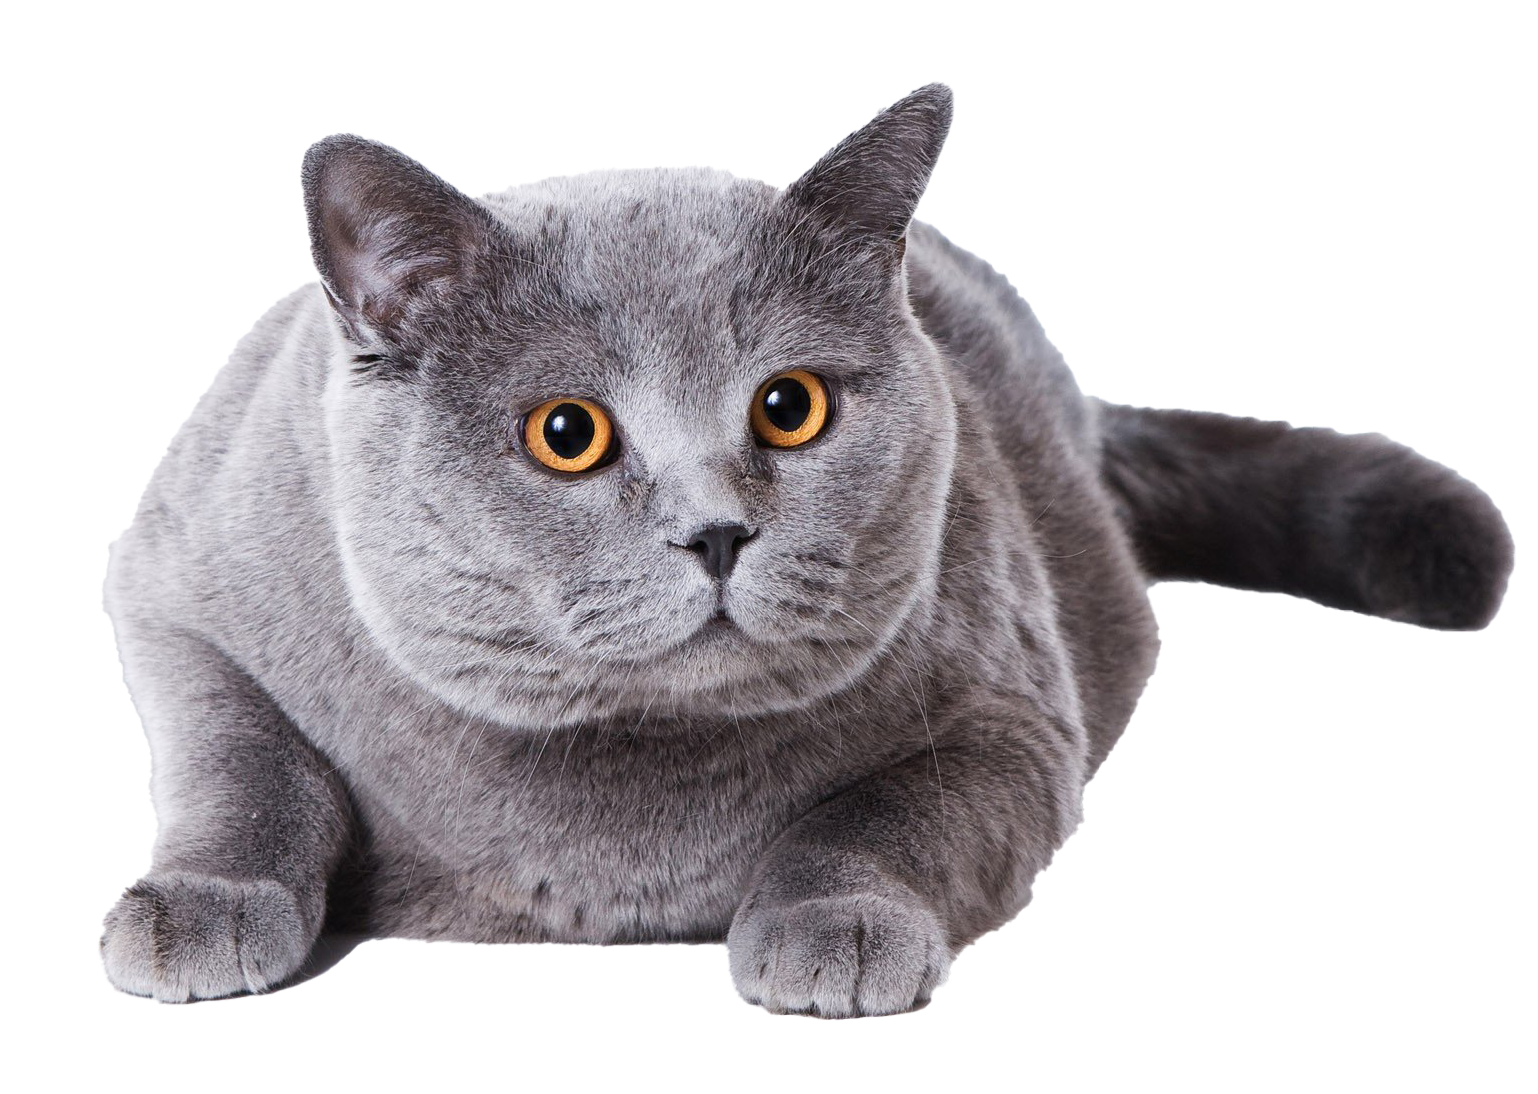
\includegraphics[width=\textwidth, angle=315]{catpng}
      \caption{Cat one}
    \end{minipage}
    \hfill
    \begin{minipage}[b]{0.4\textwidth}
      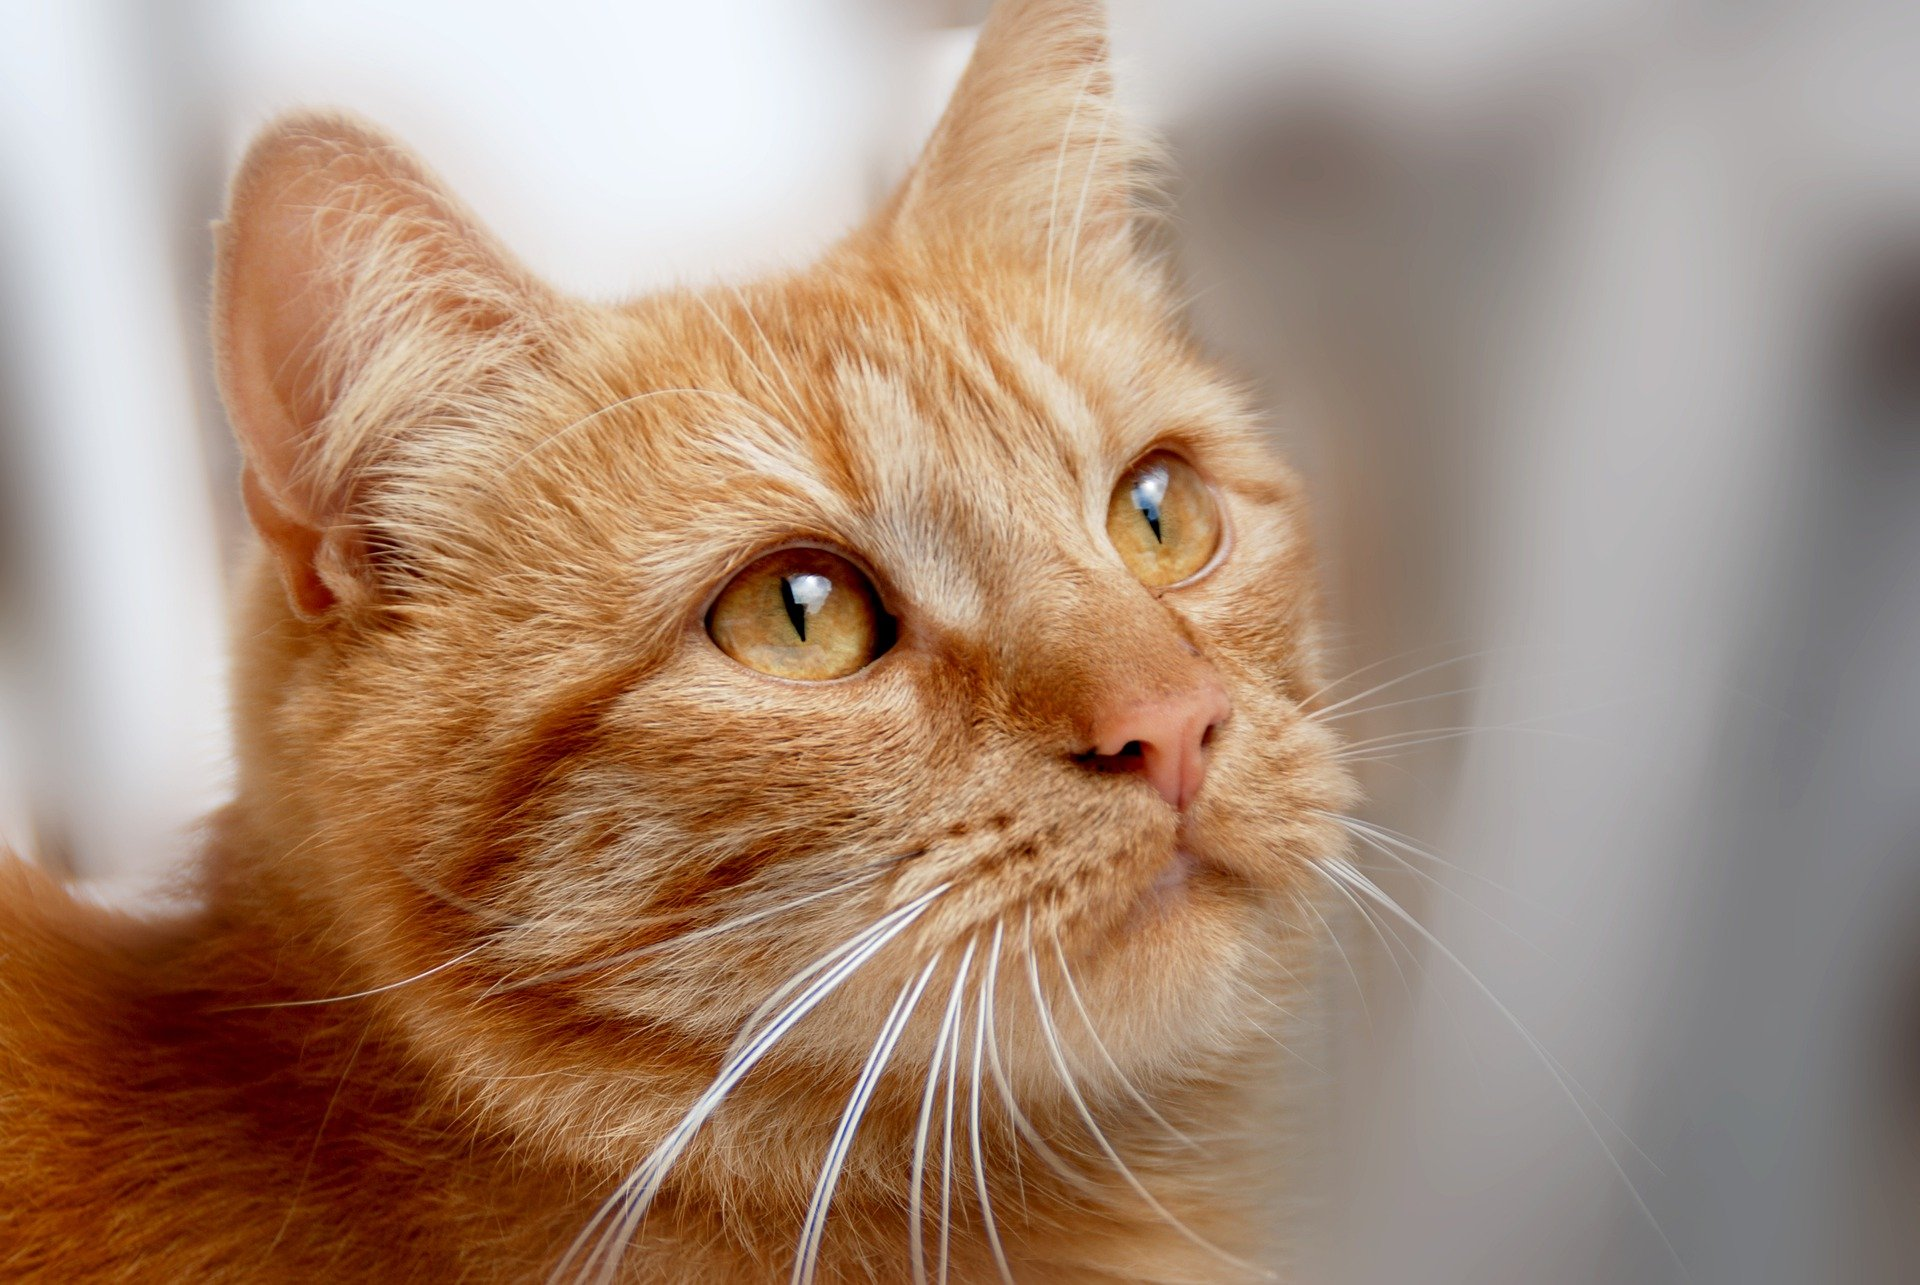
\includegraphics[width=\textwidth, angle=45]{cat.jpg}
      \caption{Cat two}
    \end{minipage}
  \end{figure}
  \ccheck{Two images next to each other}

\section{Reference to image}
Here is a reference to the centered cat: ~\ref{fig: centercat}\\
\ccheck{Image reference}

\section{Reference to page containing the image}
Here is a page reference to the centered cat: \pageref{fig: centercat}\\
\emph{(see figure \ref{fig: centercat} on page \pageref{fig: centercat})}\\
\ccheck{Image page reference}

\section{Section, subsection, subsubsection, paragraph, subparagraph}
Section text\\
\ccheck{Section}
\subsection{Subsection}
Subsection text\\
\ccheck{Subsection}
\subsubsection{Subsubsection}
Subsubsection text\\
\ccheck{Subsubsection}
\paragraph{Paragraph}
Paragraph text\\
\ccheck{Paragraph}
\subparagraph{Subparagraph}
Subparagraph text\\
\ccheck{Subparagraph}


\subsection{Numbered section}
Numbered section text\\
\ccheck{Numbered section}

\subsection*{Non-numbered section}
Non-numbered section text\\
\ccheck{Non-numbered section}

\section{Lists}

\subsection{Bullet points}
\begin{itemize}
    \item Bullet point one
    \item Bullet point two
    \item Bullet point three
  \end{itemize}
\ccheck{Bullet points}

\subsection{Alternative bullet symbols}
\begin{itemize}
    \item  Default bullet point
    \item[$\blacksquare$]  Black square for second entry
    \item[$\square$]  Square for third entry
    \item[$\textendash$] Dash for fourth entry
   \end{itemize}
\ccheck{Alternative bullet symbols}

\subsection{Enumerated lists}

\begin{enumerate}
    \item Enumerated entry one
    \item Enumerated entry two
    \item Enumerated entry three
  \end{enumerate}
\ccheck{Enumerated lists}

\subsubsection{Alternatively numbered lists}
\renewcommand{\labelenumi}{\Roman{enumi}}
\begin{enumerate}
    \item (modified) Enumerated entry one
    \item (modified) Enumerated entry two
    \item (modified) Enumerated entry three
  \end{enumerate}
\ccheck{Alternatively numbered lists}

\section{Table}
%https://www.latex-tutorial.com/tutorials/tables/
\subsection{Various horizontal alignments in columns (l, r, c)}
\begin{table}[h!]
  \begin{center}
    \begin{tabular}{l r c} % left, right, center
      \textbf{Left} & \textbf{Right} & \textbf{Center}\\
      \hline
      1 & 1110.1 & a\\
      2 & 10.1 & b\\
      3 & 23.113231 & c\\
    \end{tabular}
  \end{center}
\end{table}
\ccheck{Various horizontal alignments}

\subsection{Cell spanning multiple columns}
\begin{table}[h!]
  \begin{center}
    \begin{tabular}{l|r|c}
      \textbf{Left} & \textbf{Right} & \textbf{Center}\\
      \hline
      %multicolumn{NUMBER_OF_COLUMNS}{ALIGNMENT}{CONTENT}
      \multicolumn{2}{c|}{multicolumn} & a\\ % <-- Combining two cells with alignment c| and content 12.
      \hline
      2 & 10.1 & b\\
      3 & 23.113231 & c\\
      4 & 25.113231 & d\\
    \end{tabular}
  \end{center}
\end{table}
\ccheck{Cell spanning multiple columns}

\subsection{Vertical alignment in multi-line cells}
No solution

\subsection{Table description and label}
\begin{table}[H]
  \begin{center}
    \caption{Multirow and -column table.}
    \label{tab:table1}
    \begin{tabular}{l|c|r}
      \textbf{Value 1} & \textbf{Value 2} & \textbf{Value 3}\\
      $\alpha$ & $\beta$ & $\gamma$ \\
      \hline
      \multicolumn{2}{c|}{\multirow{2}{*}{1234}} & a\\ % <-- Multicolumn spanning 2 columns, content multirow spanning two rows
      \multicolumn{2}{c|}{} & b\\ % <-- Multicolumn spanning 2 columns with empty content as placeholder
      \hline
      3 & 23.113231 & c\\
      4 & 25.113231 & d\\
    \end{tabular}
  \end{center}
\end{table}
\ccheck{Table description and label}

\subsection{Reference to table}
See table \ref{tab:table1} on page \pageref{tab:table1}.\\
\ccheck{Reference to table}


\section{Code}
\subsection{Syntax highlighting}
\begin{minted}[linenos, bgcolor=lightgray, xleftmargin=\parindent]{html}
  <!DOCTYPE html>
  <html>
     <head>
         <title>Hello</title>
     </head>
     <body>Hello World</body>
  </html>
\end{minted}
%\subsection{Sample Java code}

\lstset{
tabsize = 4, 
showstringspaces = false, 
numbers = left, 
commentstyle = \color{gray}, 
keywordstyle = \color{blue}, 
stringstyle = \color{olive}, 
rulecolor = \color{white}, 
basicstyle = \small \ttfamily , 
breaklines = true, 
numberstyle = \small,
}

\begin{lstlisting}[language = Java , firstnumber = last , escapeinside={(*@}{@*)}]
package starshipfunctionality;

public class Starship implements DrawListener {
   
    private Draw draw = new Draw();
    private double rx, ry;        // position
    private double vx, vy;        // velocity
    private double direction;     // orientation of ship

    public Starship() {
        draw.addListener(this);
        show();
        draw.setPenColor(Color.WHITE);
        draw.text("Press 'w', 'a', 's' or 'd' to move");
        draw.show(1000);
    }

    public void launch() {
        rx = ry = 0.5;
        vx = vy = 0.0;
        direction = 0.0;

        while (true) {
            rx = rx + vx;
            ry = ry + vy;
            show();
            draw.show(50);
        }
    }
}
\end{lstlisting}
 % shit dont work

\section{Math equations}
\subsection{Inline equations}
The well known Pythagorean theorem \(x^2 + y^2 = z^2\) was 
proved to be invalid for other exponents. 
Meaning the next equation has no integer solutions:\\
\ccheck{Inline equation}

\subsection{Equation (seperate line)}
Text before
\[ x^n + y^n = z^n \]
Text after\\
\ccheck{Equation on seperate line}

\subsection{Fractions, summations, products, roots, powers}
\textbf{Fractions} can be used alongside the text, for 
example \( \frac{1}{2} \), and in a mathematical 
display style like the one below:
\[\frac{1}{2}\]
\ccheck{Fractions}\\

\textbf{Summations} can be used alongside the text, for 
example $\sum_{n=1}^{\infty} 2^{-n} = 1$ inside text, and in a mathematical 
display style like the one below:
\[ \sum_{n=1}^{\infty} 2^{-n} = 1 \]
\ccheck{Summations}\\

\textbf{Products} can be used alongside the text, for 
example $\prod_{i=a}^{b} f(i)$ inside text, and in a mathematical 
display style like the one below:
\[ \prod_{i=a}^{b} f(i) \]
\ccheck{Products}\\

\textbf{Roots} can be used alongside the text, for 
example $\frac{-b \pm \sqrt{b^2 - 4ac}}{2a}$ inside text, and in a mathematical 
display style like the one below:
\[ \frac{-b \pm \sqrt{b^2 - 4ac}}{2a} \]
\ccheck{Roots}\\

\textbf{Exponents} can be used alongside the text, for 
example ${2^2}$ inside text, and in a mathematical 
display style like the one below:
\[ {2^2} \]
\ccheck{Exponents}\\


\section{Bibliography with book, article and internet link}
Book: \cite{bookbib}\\ \ccheck{Book citation}\\
Article: \cite{articlebib}\\ \ccheck{Article citation}\\
Internet: \cite{internetbib}\\ \ccheck{Internet citation}\\

\bibliographystyle{plain}
\bibliography{bibliography} 

\section{Todo notes of own choice}
\thispagestyle{empty} % no numbering [second page] (better than gobble)
\begin{CheckList}{Task}
  \Task{done}{Title page without page number}
  \Task{done}{Table of contents}
  \Task{done}{Danish characters}
  \Task{done}{Image}
  \Task{done}{Caption over image}
  \Task{done}{Caption under image}
  \Task{done}{Image Label}
  \Task{done}{Centering}
  \Task{done}{Two images next to each other}
  \Task{done}{Reference to image}
  \Task{done}{Reference to page containing the image}
  \Task{done}{Section, subsection, subsubsection, paragraph, subparagraph}
  \Task{done}{Numbered section}
  \Task{done}{Non-numbered section}
  \Task{done}{Bullet point List}
  \Task{done}{Alternative bullet symbols List}
  \Task{done}{Enumerated Lists}
  \Task{done}{Alternatively numbered lists (roman numerals, letters)}
  \Task{done}{Table with multiple columns}
  \Task{done}{Various horizontal alignments in columns (left, right, centered)}
  \Task{done}{Cell spanning multiple columns}
  \Task{dropped}{Vertical alignment in multi-line cells}
  \Task{done}{Table description and label}
  \Task{done}{Reference to table}
  \Task{done}{Code listing}
  \Task{done}{Code with emphasized key words in your favorite programming language}
  \Task{done}{Math equations}
  \Task{done}{Inline equations (in text)}
  \Task{done}{Display equations (on separate line)}
  \Task{done}{Fractions, summations, products, roots, powers}
  \Task{done}{Bibliography with book, article and internet link}
  \Task{done}{Todo notes of own choice}
\end{CheckList}

\end{document}